\chapter{Methods}
This chapter describes the methods used in this research.\todo[inline,
    color=red!40]{check the text in the computer settings used in simulations}% New todo added here

\section{Computational model}
\textit{Description of the model implementation.}

The network model that was used in this research is a custom implementation
made by \textcite{sanjayImpairedDendriticInhibition2015}. This model is based
on the CA3 subfield region of the hippocampus and is implemented in the NEURON
simulation environment using python version 3.9.16 as an interface
\href{https://www.neuron.yale.edu}{(\url{https://www.neuron.yale.edu)}}. The
model consists of 1000 neurons, which are divided into populations of 800
pyramidal cells and 200 soma-inhibiting basket cells and 200 Oriens-Lacunosum
Moleculare (O-LM) interneurons. The implementation used in this research made
in cooperation with Sean Gies is part of the \textit{Neuromics} software
package by Synaptica Ltd.

\begin{figure}[htbp]
    \centering
    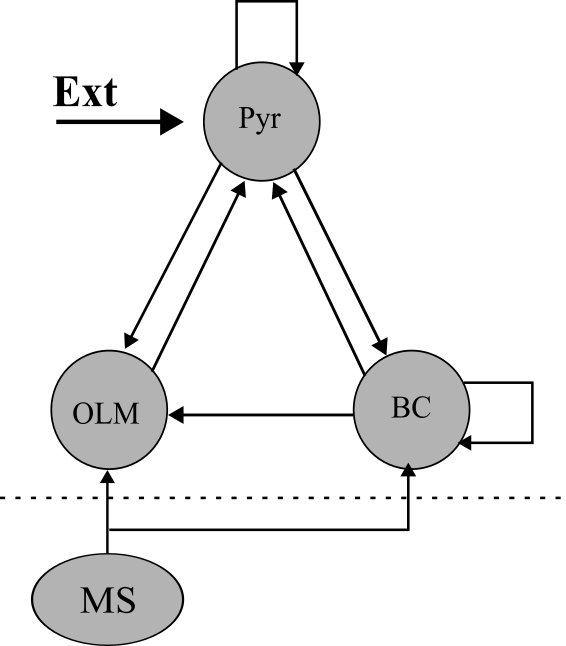
\includegraphics[width=0.5\textwidth]{model_design.png}
    \caption[Schematic of the CA3 network model]{Schematic of the CA3 network model.}
    \begin{minipage}{0.9\textwidth}
        The network comprises of many microcircuits with the connectivity as shown in the above figure. Pyr cells (pyramidal), BC cells (basket cells that inhibit soma),
        OLM cells (oriens lacunosum moleculare interneurons that inhibit dendrites), external inputs (mainly from the entorhinal cortex) to Pyr cells, and MS (medial septum).
        BC and OLM cells are stimulated by Pyr cells, while Pyr cells are inhibited by BC and OLM cells.
        Recurrent connections among Pyr cells are excitatory, whereas those among BC cells are inhibitory.
        OLM cells are inhibited by BC cells. The medial septum (MS) delivers inhibitory inputs every 150 ms to BC and OLM cells.
    \end{minipage}\label{fig:model_design}
\end{figure}\pagebreak

This is a test reference to figure~\ref{fig:model_design}, see it works!%remove later

\section{Model implementation: cell parameters}
The model consists of three types of neurons, each with its own set of
parameters and defined cell classes. The parameters for each cell type are
based on the following references:
\begin{enumerate}
    \item \textbf{Basket Cells}: Modeled after \textcite{wangGammaOscillationSynaptic1996},
          featuring standard dynamics for Na and K currents, along with synaptic and leak currents.
          Each cell is modeled as a single compartment and obeys the following current balance equation:
          \begin{equation}
              C_I \frac{dV_I}{dt} = I_{\text{app},I} - I_{\text{Na},I} - I_{\text{K},I} - I_{\text{L},I} - I_{\text{syn},I}
          \end{equation}

          where \(V_I\) is the membrane potential (mV), \(C_I = 1 \, \mu\text{F/cm}^2\)
          is the membrane capacitance, \(I_{\text{app},I}\) is the applied current, and
          \(I_{\text{syn},I}\) is the total synaptic current. The leak current
          \(I_{\text{L},I} = g_{\text{L},I}(V_I - E_{\text{L},I})\) has a conductance
          \(g_{\text{L},I} = 0.1 \, \text{mS/cm}^2\) and reversal potential
          \(E_{\text{L},I} = -65 \, \text{mV}\). All currents are in units of
          \(\mu\text{A/cm}^2\). The sodium \(I_{\text{Na},I}\) and potassium
          \(I_{\text{K},I}\) currents are voltage-dependent spiking currents of the
          Hodgkin-Huxley type.
    \item \textbf{O-LM Cells}: Adapted from \textcite{saragaActiveDendritesSpike2003},
          including additional currents like hyperpolarization-activated (h) and A-type currents.
          Each cell is modeled as a single compartment and obeys the following current balance equation:
          \begin{equation}
              C_O \frac{dV_O}{dt} = I_{\text{app},O} - I_{\text{Na},O} - I_{\text{K},O} - I_{\text{L},O} - I_{\text{h},O} - I_{\text{A},O} - I_{\text{syn},O}
          \end{equation}

          where \(V_O\) is the membrane potential, \(C_O = 1.3 \, \mu\text{F/cm}^2\) is
          the membrane capacitance, \(I_{\text{app},O}\) is the applied current, and
          \(I_{\text{syn},O}\) is the total synaptic current. The leak current
          \(I_{\text{L},O} = g_{\text{L},O}(V_O - E_{\text{L},O})\) with conductance
          \(g_{\text{L},O} = 0.05 \, \text{mS/cm}^2\) and reversal potential
          \(E_{\text{L},O} = -70 \, \text{mV}\). \(I_{\text{Na},O}\), \(I_{\text{K},O}\),
          \(I_{\text{h},O}\), and \(I_{\text{A},O}\) represent the transient sodium,
          delayed rectifier potassium, hyperpolarization-activated (or h) mixed-cation,
          and A-type potassium currents, respectively, all in units of
          \(\mu\text{A/cm}^2\).
    \item \textbf{Pyramidal Cells}: Based on \textcite{miglioreDendriticIhSelectivelyBlocks2004},
          incorporating compartmentalized dynamics for the complex morphology of pyramidal neurons.
          Each cell is modeled as a multi-compartmental neuron with 5 compartments: 1 for basal dendrites (Bdend),
          1 for soma, and 3 for apical dendrites (Adend1, 2 and 3). Each compartment obeys the following current balance equation:
          \begin{equation}
              C_{E_k} \frac{dV_{E_k}}{dt} = I_{\text{app},E_k} - I_{\text{Na},E_k} - I_{\text{K},E_k} - I_{\text{L},E_k} - I_{\text{h},E_k} - I_{\text{A},E_k} - I_{\text{syn},E_k} + I_{\text{conn},E_k}
          \end{equation}

          where \(V_{E_k}\) is the membrane potential of compartment \(k\), \(C_{E_k}\)
          is the membrane capacitance, \(I_{\text{app},E_k}\) is the applied current,
          \(I_{\text{syn},E_k}\) is the total synaptic current, and
          \(I_{\text{conn},E_k}\) represents the current due to electrical coupling
          between compartments. \(I_{\text{L},E_k}\), \(I_{\text{Na},E_k}\),
          \(I_{\text{K},E_k}\), \(I_{\text{h},E_k}\), and \(I_{\text{A},E_k}\) denote the
          leak, transient sodium, delayed rectifier potassium,
          hyperpolarization-activated mixed-cation, and A-type potassium currents for
          compartment \(k\), respectively.

\end{enumerate}
\pagebreak

\section{Model implementation: synaptic connections}
The model contained three types of synaptic connections: excitatory, inhibitory
based on AMPA, NMDA and GABA-A receptors. Synapses were modeled by standard
NEURON double-exponential mechanism. The synaptic connections were implemented
as follows:

\begin{table}[htbp]
    \centering
    \caption[Synaptic Parameters for the Connectivity Between Neurons in the Model]{Synaptic Parameters for the Connectivity Between Neurons in the Model: Pre- and postsynaptic receptor types are given for each cell type.
        The time constants \(\tau_1\) and \(\tau_2\) are in milliseconds.
        \(\tau_1\) is the rise time constant, the time it takes for synaptic conductance to increase from baseline to peak.
        \(\tau_2\) is the decay time constant, the time it takes for the conductance to decrease from peak to baseline.
        The conductance indicates the strength of the synaptic connection and its ability to conduct ionic current across the postsynaptic membrane.
        This influences the extent to which the synaptic input can depolarize the postsynaptic neuron and is in nanoSiemens (nS).}
    \begin{tabular}{lllccc}
        \hline
        Presynaptic & Postsynaptic & Receptor & \(\tau_1\) (ms) & \(\tau_2\) (ms) & Conductance (nS) \\
        \hline
        Pyramidal   & Pyramidal    & AMPA     & 0.05            & 5.3             & 0.02             \\
        Pyramidal   & Pyramidal    & NMDA     & 15              & 150             & 0.004            \\
        Pyramidal   & Basket       & AMPA     & 0.05            & 5.3             & 0.36             \\
        Pyramidal   & Basket       & NMDA     & 15              & 150             & 1.38             \\
        Pyramidal   & OLM          & AMPA     & 0.05            & 5.3             & 0.36             \\
        Pyramidal   & OLM          & NMDA     & 15              & 150             & 0.72             \\
        Basket      & Pyramidal    & GABA-A   & 0.07            & 9.1             & 0.72             \\
        Basket      & Basket       & GABA-A   & 0.07            & 9.1             & 4.5              \\
        Basket      & OLM          & GABA-A   & 0.07            & 9.1             & 0.0288           \\
        OLM         & Pyramidal    & GABA-A   & 0.2             & 20              & 72               \\
        MS          & Basket       & GABA-A   & 20              & 40              & 1.6              \\
        MS          & OLM          & GABA-A   & 20              & 40              & 1.6              \\
        \hline
    \end{tabular}\label{tab:synaptic_parameters}
\end{table}

\section{Model implementation: stimulation and noise}
\todo[inline,
    color=red!40]{Netstim information is missing.}% New todo added here

The model was activated by external inputs originating from the entorhinal
cortex, which were then transmitted to the pyramidal cells. Background random
excitatory and inhibitory inputs were received by the OLM, basket cells, and
the soma of the pyramidal cells via their AMPA, NMDA, and GABA-A receptors as
shown in table~\ref{tab:synaptic_parameters}. Similarly, the distal dendritic
compartments of the pyramidal cells also received comparable inputs through the
same types of receptors. Connections such as OLM to pyramidal cell, basket to
pyramidal cell, basket-basket recurrent connections, and medial septum to OLM
and basket cell connections were mediated through GABA-A receptors.
Additionally, the medial septum provided inhibitory inputs to the basket and
OLM cells at intervals of 150 ms.

\section{Simulations}
For the simulations, the model was implemented in NEURON version 7.6.3. The
simulations were run on a desktop computer with an Intel Core i7--8700K with 60
cores, GTX 4060, and 32 GB of RAM\@. Trials were run for 5000 ms with a time
integration step of 0.1 ms resulting in 50.000 simulation steps per trial
dataset. Random seeds were used to generate the external noise, connections and
cells for each trial and remained constant between trials and between
experiments. The number of trials varies between experiments and are specified
in their respective sections.

\subsection{Baseline activity}
In order to obtain baseline activity in the network as shown in figure
~\ref{fig:model_design}, current injections were added (\textbf{Pyramidal
    cells:} 50 pA\@; \textbf{OLM cells:} -25 pA). At Baseline, the network
generates theta-modulated gamma oscillations activity. This activity was
measured from the Local Field potential (LFP) in the network. The LFP was
simulated by a sum difference between membrane potential of the distal apical
and basal dendritic compartment over all pyramidal cells. As discussed in the
cell parameters section, all cells contained leak current, transient sodium
current \(I_{\text{Na}}\), and delayed rectifier current \(I_{K, \text{-}
        \text{dr}}\) to allow for action potential generation. On average, the firing
rates were \(2.36 \pm 0.024\) Hz for pyramidal cells, \(16.05 \pm 0.15\) Hz for
basket cells and \(0.96 \pm 0.027\) Hz for O-LM interneurons at baseline in the
original \parencite{sanjayImpairedDendriticInhibition2015}. However, it should
be noted that our custom implementation of the same model had a slightly
lowered baseline (see the results section). The reason for this discrepancy is
unknown and is a potential source of error in the results.

\subsection{Model validation}
In order to test the implementation of the model, results from the article were
replicated, namely figures 6A, B and C from
\textcite{sanjayImpairedDendriticInhibition2015}. In this replicated experiment
the OLM to pyramidal cells connection weight was reduced in decrements of 0.1X
times the baseline from 1.0 to 0.0. In addition to reduced connection strength,
the external noise fed into the pyramidal cells was increased in increments of
0.1X times the baseline from 1.0 to 2.0. By reducing the connectivity from OLM
to pyramidal cells, dendritic inhibition is impaired and potentially
epileptiform activity is induced. The original results focussed on three
aspects: changes in firing rates per population, the changes in dominant theta
and gamma frequencies, and finally the changes in the power of the theta and
gamma oscillations.

\subsection{Sodium and potassium variants}

\subsection{External noise variants}

\subsection{Recurrent connection strength variants}
